\chapter{Metodologia}
\label{cap:metodologia}

\section{Modello dell'ambiente}
\label{sec:ambiente}

Il bosco è modellato come un'area quadrata di 20~m di lato, delimitata da un bordo che il robot non può oltrepassare e che presenta al suo interno due differenti tipi di ostacoli: gli alberi, descritti da cerchi di raggio variabile che corrispondono alla sezione del tronco dell'albero all'altezza del sensore, e le rocce, descritte attraverso poligoni irregolari di sei vertici. Poiché il modello tiene conto solamente di questa sezione orizzontale, non sono rappresentati pendenze, irregolarità del terreno, rami e sottobosco.

Ogni bosco presenta 15 alberi e 3 rocce, generati in modo casuale estraendo il centro di ciascun ostacolo con distribuzione uniforme nell'area. Il raggio di ciascun albero è estratto casualmente tra 0,3 e 1~m, mentre per le rocce si estrae una dimensione tra 0,4 e 1~m e si dispongono i sei vertici a intervalli angolari regolari attorno al centro, ciascuno a una distanza compresa tra il 60\% e il 100\% di tale dimensione, in modo che la forma risulti irregolare. Un ostacolo viene accettato, cioè considerato come ostacolo valido per il bosco considerato, solo se è interamente contenuto nell'area, non interseca gli ostacoli già presenti e dista almeno 1,5~m dal punto di partenza del robot. Nel caso in cui tali condizioni non fossero rispettate la sua posizione viene estratta di nuovo, fino a un massimo di 100 tentativi. Nei boschi usati per i test nessun ostacolo esaurisce i tentativi disponibili, per cui i 18 ostacoli vengono sempre inseriti tutti e occupano in media il 5,8\% dell'area complessiva; un esempio è riportato nella Figura~\ref{fig:bosco}.

La generazione dipende da un seme numerico (\textit{seed}) e lo stesso seme produce sempre lo stesso bosco. Questo approccio ha garantito la riproducibilità dei test, cioè la possibilità di ripetere un esperimento nelle stesse condizioni e di confrontare strategie diverse sugli stessi boschi. La distanza minima impostata rispetto al punto di partenza serve invece a evitare che il robot inizi l'esplorazione a ridosso di un ostacolo. Come punto di partenza per le esplorazioni si è scelto di utilizzare il centro dell'area oppure, in una seconda serie di test, il suo angolo in basso a sinistra (Sezione~\ref{sec:protocollo}).

Il bosco così generato è dunque la realtà di riferimento della simulazione (\textit{ground truth}) e viene usato soltanto per calcolare le misure del sensore, mentre il robot conosce l'ambiente esclusivamente attraverso la mappa che costruisce progressivamente durante l'esplorazione.

Il robot, a sua volta, è modellato come un punto materiale descritto dalla sola posizione nel piano. Il suo orientamento non viene considerato, dal momento che il sensore osserva l'intero angolo giro (Sezione~\ref{sec:lidar}) e il movimento avviene tra celle adiacenti della mappa (Sezione~\ref{sec:ciclo}). Un robot reale ha però dimensioni non trascurabili, per cui si è deciso di tenere conto del suo ingombro fisico in modo indiretto e semplificato, allargando gli ostacoli nella mappa (Sezione~\ref{sec:inflazione}).

\begin{figure}[!htb]
    \centering
    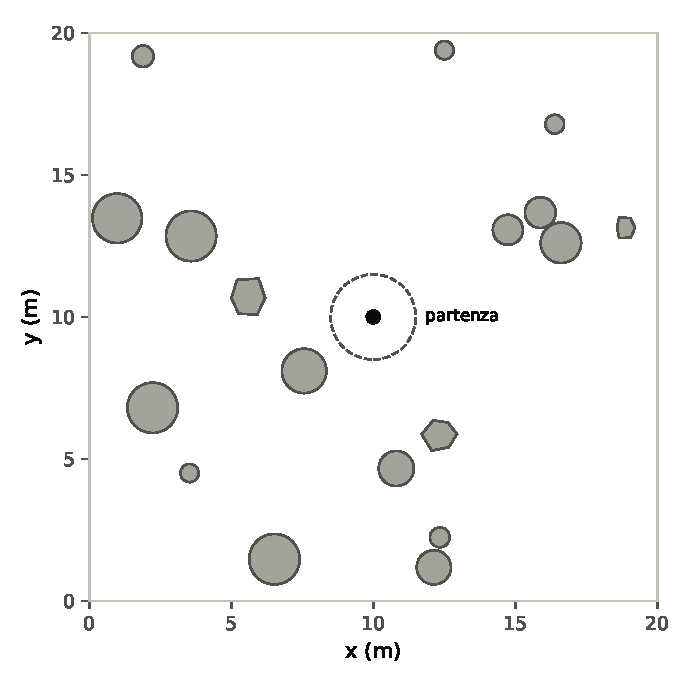
\includegraphics[width=0.6\textwidth]{bosco_esempio}
    \caption[Esempio di bosco generato]{Esempio di bosco generato (seed 44): 15 alberi, rappresentati da cerchi, e 3 rocce, rappresentate da esagoni irregolari, in un'area di 20 $\times$ 20~m. Il punto nero è la posizione di partenza del robot al centro dell'area; il cerchio tratteggiato delimita la zona di raggio 1,5~m in cui non vengono collocati ostacoli.}
    \label{fig:bosco}
\end{figure}

\section{Modello del sensore LiDAR}
\label{sec:lidar}

Il sensore è un LiDAR bidimensionale che misura le distanze nel piano orizzontale in corrispondenza dell'altezza alla quale è montato. Il modello che è stato impiegato in questo lavoro è quello sviluppato in~\cite{gennai2026} e riutilizzato come strumento per effettuare le varie scansioni oggetto degli esperimenti.

Ogni scansione è composta da 360 raggi che partono dalla posizione del robot e sono distribuiti uniformemente sull'angolo giro, con un passo di circa 1\textdegree. Ciascun raggio è un segmento lungo quanto la portata massima del sensore, fissata a 4~m, di cui si cerca la prima intersezione con gli ostacoli. Se questa esiste, il sensore restituisce il punto colpito, che si trova sul contorno perimetrale di un albero o di una roccia, altrimenti restituisce il punto finale del raggio, a 4~m dal robot. Il bordo dell'area non viene rilevato dalle scansioni, di conseguenza i raggi diretti verso di esso proseguono fino alla portata massima. Dato che ogni raggio si ferma non appena incontra il contorno di un determinato ostacolo, la zona alle spalle di un tronco o di una roccia resta inosservata finché il robot non la vede da un'altra posizione, cioè da un'angolazione differente rispetto alla precedente scansione, come si nota nella Figura~\ref{fig:scansione}, che rappresenta una scansione eseguita dal punto di partenza.

In questo lavoro si è scelto di lavorare in condizioni ideali, quindi le misure sono prive di rumore e la distanza restituita coincide con quella esatta tra il robot e il punto colpito. Il modello impiegato permetterebbe di aggiungere un rumore gaussiano alle distanze, rendendo così la simulazione più realistica, possibilità questa che non è stata usata o approfondita in questo lavoro.

Ne risulta che una scansione contiene due tipi di raggi, che forniscono informazioni diverse. Un raggio che colpisce un ostacolo dà la posizione di un punto del suo perimetro e indica che lo spazio tra il robot e quel punto è libero, mentre un raggio che non colpisce nulla indica soltanto che lo spazio è libero fino alla portata massima. Entrambe le informazioni vengono usate per costruire la mappa (Sezione~\ref{sec:aggiornamento}). I punti colpiti, raccolti a ogni scansione, formano inoltre la nuvola di punti accumulata durante l'esplorazione, che in un'applicazione reale è il dato da cui stimare la posizione e il diametro dei tronchi.

\begin{figure}[!htb]
    \centering
    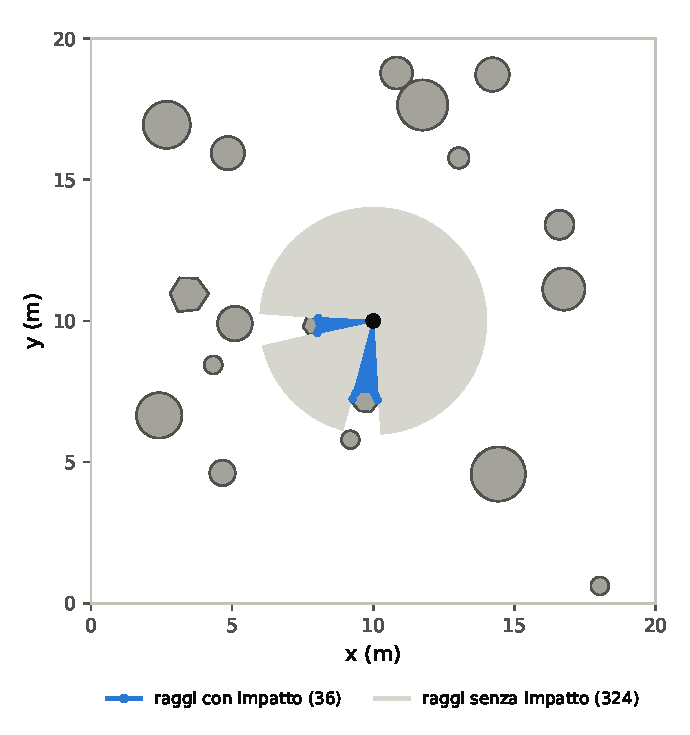
\includegraphics[width=0.6\textwidth]{scansione_lidar}
    \caption[Scansione LiDAR dal punto di partenza]{Scansione LiDAR dal punto di partenza nel bosco della Figura~\ref{fig:bosco}. In blu i raggi che colpiscono un ostacolo, con il punto di impatto; in grigio chiaro i raggi che raggiungono la portata massima di 4~m senza incontrare ostacoli. La roccia e l'albero vicini al robot nascondono le zone alle loro spalle.}
    \label{fig:scansione}
\end{figure}

\section{Mappa a griglia di occupazione}
\label{sec:mappa}

Il robot descrive la propria conoscenza dell'ambiente con una mappa a griglia di occupazione~\cite{elfes1989}, che suddivide l'area in celle quadrate di 0,2~m di lato, per un totale di 100 $\times$ 100 celle, e associa a ciascuna uno specifico stato. Nella formulazione originale ogni cella contiene una probabilità di occupazione, aggiornata a ogni misurazione per tenere conto del rumore del sensore. Poiché in questo lavoro le misure sono esatte, si usa invece uno stato discreto, aggiornato secondo regole deterministiche. All'inizio dell'esplorazione tutte le celle sono sconosciute, e la mappa viene completata progressivamente con le scansioni eseguite dal robot.

\subsection{Stati delle celle}
\label{sec:stati}

Ogni cella si trova in uno di quattro stati distinti. Una cella è sconosciuta finché nessuna scansione l'ha osservata, libera quando una scansione l'ha riconosciuta come priva di ostacoli secondo le regole della Sezione~\ref{sec:aggiornamento}, e occupata quando contiene il punto colpito da un raggio. Il quarto stato, detto di sicurezza, riguarda le celle libere troppo vicine a un ostacolo perché il robot possa occuparle senza urtarlo, e si ottiene allargando gli ostacoli come descritto nella Sezione~\ref{sec:inflazione}. Ai fini del movimento conta soltanto la distinzione tra le celle libere, le sole percorribili, e tutte le altre, per cui il robot non entra mai in una cella sconosciuta, occupata o di sicurezza. Nelle figure di questo lavoro i quattro stati sono disegnati rispettivamente in grigio, bianco, nero e rosso.

\subsection{Griglia locale e aggiornamento della mappa globale}
\label{sec:aggiornamento}

Ogni scansione viene prima tradotta in una griglia locale, centrata sulla posizione del robot e di lato pari al doppio della portata del sensore, cioè 8~m, così da contenere tutti i punti che la scansione può raggiungere. La griglia locale ha la stessa risoluzione della mappa globale e parte con tutte le celle sconosciute. Ciascun raggio viene poi campionato verso la sua estremità a intervalli regolari di un quarto di cella, le celle in cui cadono i campioni vengono segnate come libere e, se il raggio ha colpito un ostacolo, la cella che contiene il punto colpito viene segnata come occupata. Il tratto segnato come libero non arriva fino all'estremità del raggio, per i motivi discussi nella Sezione~\ref{sec:margini}.

La griglia locale viene poi fusa nella mappa globale secondo tre regole: le celle locali sconosciute non portano informazione e vengono ignorate, una cella globale ancora sconosciuta assume lo stato indicato dalla griglia locale, mentre una cella globale già nota cambia stato solo se la griglia locale la indica come occupata. Date queste regole adottate ne consegue che una cella libera può diventare occupata quando una scansione successiva vi rileva al suo interno un ostacolo, mentre una cella occupata non torna mai libera. Tale scelta adottata è coerente con un sensore privo di rumore, per il quale un punto colpito corrisponde sempre a un ostacolo reale, privilegiando in questo modo la sicurezza, dal momento che rispetto alle informazioni già presenti nella mappa globale prevale sempre quella che vieta il passaggio. Dopo ogni fusione gli ostacoli vengono allargati come descritto nella Sezione~\ref{sec:inflazione}.

\subsection{Margini sullo spazio libero}
\label{sec:margini}

Segnare come libere tutte le celle attraversate da un raggio porterebbe a considerare libere anche celle che contengono una parte di ostacolo. Una cella ha un lato di 0,2~m e può essere attraversata da un raggio anche quando un ostacolo ne occupa una porzione che il raggio non interseca. Questo fenomeno, che andrebbe a compromettere la sicurezza degli spostamenti del robot durante la sua esplorazione, accade soprattutto per i raggi radenti, che sfiorano il contorno di un tronco con un angolo piccolo e ne attraversano le celle sul fianco prima di colpirlo, oppure senza colpirlo affatto. Per limitare il problema, il tratto segnato come libero viene accorciato in modo diverso a seconda del tipo di raggio interessato.

Per un raggio che colpisce un ostacolo, le celle vengono segnate libere solo fino a 0,2~m prima del punto colpito, cioè fino a una cella prima. Questa distanza è indicata nel seguito come margine sul libero. Per un raggio che non colpisce nulla, invece, le celle vengono segnate libere solo fino a 3,4~m, lasciando sconosciuta una corona di sicurezza di 0,6~m all'estremità della portata. La corona, introdotta su indicazione del relatore, tiene conto del fatto che la distanza tra due raggi adiacenti cresce allontanandosi dal robot e raggiunge circa 7~cm alla portata massima. Vicino a questa distanza una cella può quindi contenere una parte di ostacolo che nessun raggio raggiunge, perché cade tra due raggi o appena oltre la loro estremità, e verrebbe segnata libera per errore. Lasciandola sconosciuta, la cella viene classificata solo quando il robot si avvicina e la osserva da una distanza minore che gli permette quindi di avere una visione più completa e sicura dell'ostacolo. Lo spessore di 0,6~m è stato scelto confrontando i valori 0, 0,2, 0,4 e 0,6~m su cinque boschi differenti, come compromesso tra la riduzione degli errori e la parte di portata che la corona sottrae alla classificazione delle celle.

Nessuno dei due margini elimina del tutto il problema. Quando una cella segnata libera da lontano viene osservata da vicino, la nuova scansione può rilevarvi un ostacolo, per cui la cella diventa occupata e l'allargamento degli ostacoli rende di sicurezza anche le celle libere adiacenti. Questo fenomeno, indicato nel seguito come scoperta tardiva, riguarda soprattutto il fianco dei tronchi o delle rocce osservato con raggi radenti e ha due conseguenze: il percorso già seguito dal robot può risultare, a posteriori, sovrapposto a celle che nel frattempo sono diventate di sicurezza, anche se al momento del passaggio erano libere, e il robot può ritrovarsi in una posizione da cui non è più possibile raggiungere alcuna frontiera, situazione analizzata nel Capitolo~\ref{cap:risultati}.

\subsection{Inflazione degli ostacoli}
\label{sec:inflazione}

Il robot è modellato come un punto materiale adimensionale, ma un robot reale ha un ingombro e non può avvicinarsi a un ostacolo fino a toccarlo. Per tenerne conto in modo semplificato, dopo ogni aggiornamento della mappa globale ogni cella libera che dista non più di 0,2~m da una cella occupata, misurando la distanza tra i centri delle celle, passa nello stato di sicurezza. Con la risoluzione adottata questo raggio corrisponde a una cella, per cui diventano di sicurezza le quattro celle adiacenti a ogni cella occupata. Una cella di sicurezza non torna più libera e non è percorribile, quindi i percorsi pianificati si mantengono a distanza dagli ostacoli. Il bordo dell'area, invece, non è un ostacolo e non viene conseguentemente allargato, per cui il robot può muoversi anche nelle celle a contatto con il bordo.

La cella in cui si trova il robot è esclusa da questa regola e viene inoltre forzata nello stato libero dopo ogni aggiornamento. Senza questa eccezione, un ostacolo scoperto vicino al robot potrebbe rendere non libera la sua stessa cella, che è il punto di partenza di ogni pianificazione, e il robot non avrebbe più un percorso valido attraverso cui proseguire durante la sua esplorazione. La forzatura è giustificata dal fatto che il robot si trova al centro della propria cella e vi è arrivato attraversando celle libere, seguendo dunque un percorso valido e percorribile fisicamente, per cui la sua posizione è effettivamente fuori dagli ostacoli anche quando una parte della cella risulta occupata.

La Figura~\ref{fig:mappa} mostra la mappa ottenuta dalla prima scansione eseguita dal punto di partenza, in cui sono visibili gli elementi descritti in questa sezione.

\begin{figure}[!htb]
    \centering
    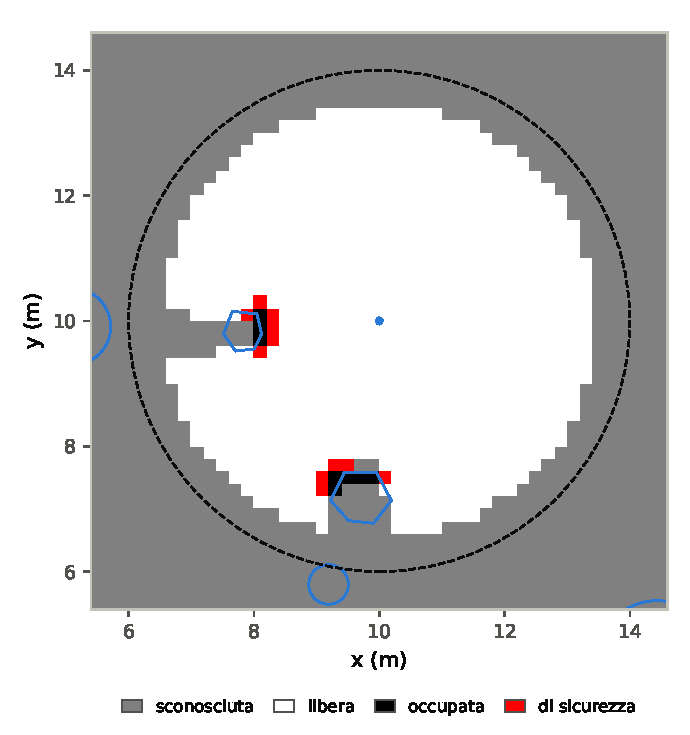
\includegraphics[width=0.6\textwidth]{mappa_prima_scansione}
    \caption[Mappa dopo la prima scansione]{Mappa dopo la prima scansione dal punto di partenza, ingrandita attorno al robot, per il bosco della Figura~\ref{fig:bosco}. Le celle libere formano un disco di raggio 3,4~m, e l'anello sconosciuto che lo separa dal cerchio tratteggiato, corrispondente alla portata di 4~m, è la corona. Le celle occupate si trovano sul contorno della roccia e dell'albero colpiti dalla scansione, il cui profilo reale è tracciato in blu insieme alla posizione del robot, e sono affiancate dalle celle di sicurezza, mentre le zone alle spalle dei due ostacoli restano sconosciute.}
    \label{fig:mappa}
\end{figure}

\section{Frontiere e raggiungibilità}
\label{sec:frontiere}

Seguendo la definizione di Yamauchi~\cite{yamauchi1997}, una frontiera è una cella libera che confina con almeno una cella sconosciuta, dove le celle confinanti sono le quattro che condividono un lato con essa. Le frontiere segnano il limite della parte di ambiente già osservata e sono le destinazioni candidate dell'esplorazione. Quando il robot raggiunge una frontiera, la scansione eseguita da quella posizione osserva almeno in parte le celle sconosciute vicine garantendo un'espansione della mappa conosciuta. Le celle esterne all'area non contano come sconosciute, per cui il bordo non genera frontiere.

Una frontiera può essere utile come destinazione solo se il robot è in grado di raggiungerla. Prima di ogni scelta della destinazione si determinano quindi le celle raggiungibili dalla posizione del robot, esplorando la mappa a partire dalla sua cella e passando da una cella libera a un'altra confinante, sempre attraverso un lato di essa. In questo modo si ottiene, per ogni cella raggiungibile, anche la sua distanza dal robot, misurata come numero minimo di passi tra celle libere. Questa distanza tiene conto degli ostacoli e delle zone non ancora osservate, per cui può essere molto maggiore della distanza in linea d'aria, ed è la misura usata dalle strategie che scelgono la destinazione in base alla vicinanza (Sezione~\ref{sec:strategie}).

Alle strategie viene passato solo l'insieme delle frontiere raggiungibili, da cui sono escluse due categorie di celle. La prima è la cella in cui si trova il robot, che può risultare una frontiera poiché viene forzata nello stato libero (Sezione~\ref{sec:inflazione}) e che non avrebbe senso scegliere come destinazione. La seconda comprende le frontiere che il robot ha già raggiunto senza che smettessero di essere tali, per esempio perché una cella sconosciuta adiacente si trova all'interno di un ostacolo o in una zona che nessun raggio riesce a raggiungere. Senza questa esclusione il robot potrebbe sceglierle di nuovo indefinitamente. Quando non esiste alcuna frontiera l'esplorazione è completa, mentre quando esistono frontiere ma nessuna è raggiungibile il robot si ferma. Il significato di questa seconda condizione è discusso nella Sezione~\ref{sec:ciclo}.

\section{Pianificazione del percorso}
\label{sec:pianificazione}

Una volta scelta la destinazione, il percorso per raggiungerla viene calcolato con l'algoritmo di Dijkstra~\cite{dijkstra1959}, applicato a un grafo i cui nodi sono le celle libere della mappa e gli archi collegano le celle libere che condividono un lato. Ogni arco ha lo stesso costo, pari allo spostamento di una cella, per cui il percorso restituito è una sequenza di celle libere adiacenti che collega la cella del robot alla destinazione con il minor numero possibile di passi. Il robot si muove quindi solo nelle quattro direzioni parallele ai lati della griglia, e ogni passo corrisponde a uno spostamento di 0,2~m.

Poiché il grafo contiene soltanto celle libere, il percorso non attraversa mai celle sconosciute, occupate o di sicurezza. La pianificazione si basa esclusivamente sulla parte di ambiente già osservata e riconosciuta come percorribile. Un percorso verso la destinazione esiste sempre, dato che questa viene scelta tra le frontiere raggiungibili e la verifica di raggiungibilità (Sezione~\ref{sec:frontiere}) si muove sulle stesse celle libere e con gli stessi spostamenti usati dalla pianificazione.

Con costi tutti uguali l'algoritmo di Dijkstra visita le celle nello stesso ordine di una ricerca in ampiezza e fornisce lo stesso risultato, per cui la lunghezza del percorso pianificato coincide esattamente con la distanza calcolata nella verifica di raggiungibilità. La formulazione con costi permetterebbe di assegnare agli archi pesi diversi, per esempio per penalizzare il passaggio vicino agli ostacoli, possibilità che in questo lavoro non è stata adottata. Tra i percorsi di lunghezza minima, infatti, nulla favorisce quelli lontani dagli ostacoli, e il percorso pianificato passa spesso a ridosso delle celle di sicurezza, dove la scoperta tardiva descritta nella Sezione~\ref{sec:margini} ha più probabilità di manifestarsi.

\section{Ciclo di esplorazione}
\label{sec:ciclo}

L'esplorazione procede alternando percezione, decisione e movimento, secondo lo schema della Figura~\ref{fig:ciclo}. All'inizio, e poi dopo ogni spostamento, il robot esegue una scansione dalla posizione attuale in cui è situato e aggiorna la mappa come descritto nella Sezione~\ref{sec:mappa}. I punti colpiti vengono aggiunti alla nuvola di punti e viene registrata la percentuale di area scoperta raggiunta.

Quando il robot non ha un percorso da seguire, cioè all'inizio dell'esplorazione o dopo aver raggiunto la destinazione precedente oppure dopo aver abbandonato un percorso, viene presa una nuova decisione. Si determinano le frontiere della mappa e, tra queste, quelle raggiungibili (Sezione~\ref{sec:frontiere}), dopodiché la strategia di esplorazione sceglie una di esse come destinazione e l'algoritmo di Dijkstra calcola il percorso per raggiungerla (Sezione~\ref{sec:pianificazione}).

Il percorso viene seguito progressivamente, una cella alla volta, e questo permette al robot di controllare prima di ogni spostamento che la cella successiva sia ancora libera, dato che la scansione eseguita dopo lo spostamento precedente può averla resa occupata o di sicurezza. In quel caso il percorso viene abbandonato e si torna alla scelta della destinazione, che può anche cambiare. Se invece la cella è libera, il robot si sposta al suo centro, la distanza percorsa aumenta di 0,2~m e viene eseguita una nuova scansione. La destinazione non viene rivalutata a ogni passo, per cui il robot prosegue lungo il percorso finché non la raggiunge o finché la cella successiva non risulta più libera, anche se nel frattempo la destinazione ha smesso di essere una frontiera. L'avanzamento a piccoli passi, con una scansione dopo ciascuno, permette al robot di accorgersi degli ostacoli scoperti lungo il cammino prima di attraversarli e di tornare indietro quando serve, dato che un percorso può passare per qualsiasi cella libera, comprese quelle già visitate.

L'esplorazione termina in tre casi. Se la mappa non contiene più frontiere, l'area è stata esplorata per intero, a meno delle zone che il sensore non può osservare, e l'esplorazione è completa. Se esistono frontiere ma nessuna è raggiungibile, il robot si ferma pur avendo ancora zone da esplorare. Infine, per evitare esecuzioni senza termine, l'esplorazione si interrompe forzatamente dopo 300 decisioni, un limite che nei test non è mai stato raggiunto, dato che il numero massimo di decisioni registrato è 81.

Il secondo caso corrisponde a quello che nel seguito viene chiamato blocco, e in tutti i casi analizzati ha avuto origine dallo stesso meccanismo. Il controllo eseguito prima di ogni spostamento riguarda soltanto la cella successiva e non verifica se da quella cella sarà possibile proseguire, per cui il robot può entrare in una cella la cui unica cella libera confinante è quella da cui proviene. Se la scansione eseguita dalla nuova posizione, per effetto della scoperta tardiva, rende di sicurezza anche quest'ultima, il robot resta circondato da celle non percorribili e nessuna frontiera è più raggiungibile. Nei test un'esplorazione è considerata bloccata quando termina con una copertura inferiore al 90\% (Sezione~\ref{sec:protocollo}), e l'analisi dei casi osservati è riportata nel Capitolo~\ref{cap:risultati}.

\begin{figure}[!htb]
    \centering
    % Diagramma di flusso del ciclo di esplorazione (Sezione 1.6)
\begin{tikzpicture}[
    node distance=4.5mm,
    box/.style={rectangle, draw, align=center, minimum width=50mm, minimum height=7mm, font=\small},
    side/.style={rectangle, draw, align=center, minimum width=28mm, minimum height=7mm, font=\small},
    term/.style={rectangle, draw, rounded corners=3.5mm, align=center, minimum width=28mm, minimum height=7mm, font=\small},
    dec/.style={diamond, draw, aspect=2.6, align=center, inner sep=0.5pt, font=\small},
    arr/.style={-{Stealth[length=2mm]}},
    lab/.style={font=\footnotesize}
]
    % colonna principale
    \node[term] (start) {Inizio};
    \node[box, below=of start] (scan) {Scansione e aggiornamento della mappa};
    \node[dec, below=of scan] (path) {Percorso\\da seguire?};
    \node[dec, below=of path] (front) {Esistono\\frontiere?};
    \node[dec, below=of front] (reach) {Frontiere\\raggiungibili?};
    \node[box, below=of reach] (choose) {Scelta della destinazione\\(strategia di esplorazione)};
    \node[box, below=of choose] (plan) {Calcolo del percorso (Dijkstra)};
    \node[dec, below=of plan] (next) {Cella successiva\\libera?};
    \node[box, below=of next] (move) {Spostamento di una cella};

    % esiti laterali
    \node[term] (done) at ($(front)+(58mm,0)$) {Esplorazione\\completa};
    \node[term] (block) at ($(reach)+(58mm,0)$) {Arresto\\(blocco)};
    \node[side] (drop) at ($(next)+(58mm,0)$) {Abbandono\\del percorso};

    % linee verticali dei ritorni
    \coordinate (L1) at (-37mm,0);
    \coordinate (L2) at (-44mm,0);
    \coordinate (R) at (80mm,0);
    \coordinate (J) at ($(path.south)!0.65!(front.north)$);

    % flusso principale
    \draw[arr] (start) -- (scan);
    \draw[arr] (scan) -- (path);
    \draw[arr] (path) -- node[lab, left, pos=0.3] {no} (front);
    \draw[arr] (front) -- node[lab, right] {sì} (reach);
    \draw[arr] (reach) -- node[lab, right] {sì} (choose);
    \draw[arr] (choose) -- (plan);
    \draw[arr] (plan) -- (next);
    \draw[arr] (next) -- node[lab, right] {sì} (move);

    % uscite laterali
    \draw[arr] (front) -- node[lab, above] {no} (done);
    \draw[arr] (reach) -- node[lab, above] {no} (block);
    \draw[arr] (next) -- node[lab, above] {no} (drop);

    % percorso gia' disponibile: si passa direttamente al controllo della cella successiva
    \draw[arr] (path.west) -- node[lab, above, pos=0.25] {sì} (path.west -| L1) |- (next.west);
    % dopo lo spostamento si esegue una nuova scansione
    \draw[arr] (move.west) -- (move.west -| L2) |- (scan.west);
    % dopo l'abbandono del percorso si torna alla scelta della destinazione
    \draw[arr] (drop.east) -- (drop.east -| R) |- (J);
\end{tikzpicture}

    \caption[Ciclo di esplorazione]{Ciclo di esplorazione. Dopo ogni spostamento il robot esegue una nuova scansione; la scelta della destinazione avviene solo quando non c'è un percorso da seguire, cioè all'inizio, all'arrivo a destinazione o dopo l'abbandono di un percorso. Il limite di 300 decisioni non è riportato.}
    \label{fig:ciclo}
\end{figure}

\section{Strategie di esplorazione}
\label{sec:strategie}

Una strategia di esplorazione riceve, a ogni decisione, l'insieme delle frontiere raggiungibili e la distanza di ciascuna dal robot (Sezione~\ref{sec:frontiere}), e restituisce la frontiera scelta come destinazione. Tutte le strategie operano sulla stessa mappa e affidano il calcolo del percorso allo stesso algoritmo, per cui si differenziano soltanto per il criterio con cui scelgono la destinazione. Quando più frontiere sono equivalenti rispetto al criterio di scelta impiegato dalla strategia interessata, la scelta tra di esse avviene in modo casuale. Le estrazioni dipendono dallo stesso seme usato per generare il bosco, per cui anche il comportamento delle strategie risulta di conseguenza riproducibile.

\subsection{Strategia casuale}
\label{sec:casuale}

La strategia casuale sceglie la destinazione con probabilità uniforme tra tutte le frontiere raggiungibili, senza considerare la loro distanza né la loro posizione. La scelta è casuale, ma il movimento verso la destinazione segue comunque il percorso più breve grazie all'algoritmo di pianificazione comune a tutte le strategie, per cui il robot alterna spesso spostamenti lunghi tra zone lontane dell'area. Questa strategia non usa alcuna informazione sulla struttura della mappa ed è impiegata come termine di confronto per le altre.

\subsection{Strategia basata sulle frontiere}
\label{sec:frontier}

La strategia basata sulle frontiere sceglie la frontiera raggiungibile più vicina al robot, dove la vicinanza è misurata dalla distanza lungo la griglia calcolata nella verifica di raggiungibilità. A parità di distanza la scelta è casuale. È la formulazione proposta da Yamauchi~\cite{yamauchi1997}, nella quale il robot si dirige ogni volta verso la zona sconosciuta più vicina, per cui l'esplorazione procede per spostamenti brevi e la distanza percorsa tende a essere contenuta. La scelta non tiene conto di quanto la frontiera sia vicina agli ostacoli, e le frontiere più vicine si trovano spesso proprio a ridosso dei tronchi o delle rocce, nelle zone d'ombra che il sensore non ha ancora osservato.

\subsection{Strategia a serpentina}
\label{sec:serpentina}

La strategia a serpentina si ispira agli algoritmi di copertura, e in particolare alla decomposizione \textit{boustrophedon}~\cite{choset2000}, che percorrono l'area a fasce parallele. L'area viene suddivisa in macro-celle quadrate di 4~m di lato, quindi in una griglia di 5 $\times$ 5 macro-celle, alle quali viene assegnato un ordine di visita, equivalente ad un rango di priorità. La numerazione parte dall'angolo in basso a sinistra, percorre la fascia inferiore da sinistra a destra, risale alla fascia successiva e la percorre da destra a sinistra, e così via alternando il verso fino alla fascia superiore (Figura~\ref{fig:serpentina}). A ogni decisione la strategia considera la macro-cella di ordine più basso che contiene almeno una frontiera raggiungibile e sceglie in modo casuale una delle frontiere al suo interno, senza tenere conto della distanza dal robot. In questo modo il robot completa una macro-cella prima di passare alla successiva, mentre il percorso per raggiungere la destinazione, calcolato con l'algoritmo di Dijkstra, può attraversare anche macro-celle di ordine diverso.

Il lato delle macro-celle è stato fissato a 4~m, pari alla portata del sensore, su indicazione del relatore. Una prima versione con macro-celle di 1~m costringeva il robot a percorrere l'area con un passo molto più fitto di quanto la portata del sensore richiedesse, e produceva percorsi più lunghi senza aumentare in modo rilevante la copertura dell'area esplorata.

\begin{figure}[!htb]
    \centering
    % Ordine di visita delle macro-celle nella strategia a serpentina (Sezione 1.7.3)
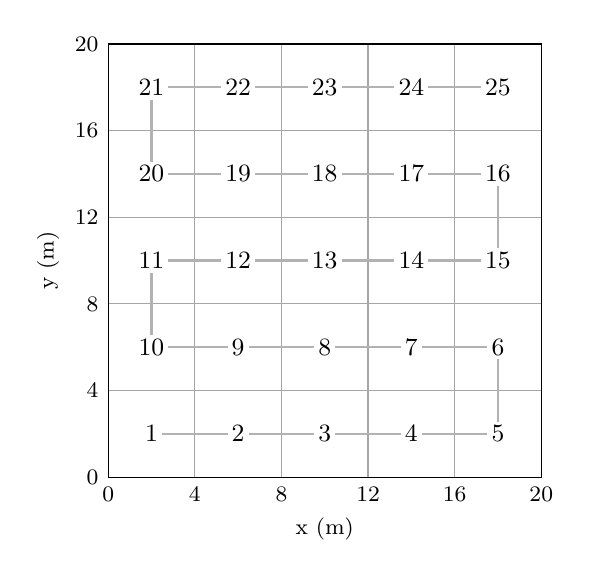
\begin{tikzpicture}[x=11mm, y=11mm, font=\small]
    % griglia 5 x 5 di macro-celle da 4 m
    \draw[step=1, gray!70] (0,0) grid (5,5);
    \draw (0,0) rectangle (5,5);

    % percorso a serpentina tra i centri delle macro-celle
    \draw[gray!60, line width=0.8pt]
        (0.5,0.5) -- (4.5,0.5) -- (4.5,1.5) -- (0.5,1.5) -- (0.5,2.5) -- (4.5,2.5)
        -- (4.5,3.5) -- (0.5,3.5) -- (0.5,4.5) -- (4.5,4.5);

    % numero d'ordine di ogni macro-cella
    \foreach \row in {0,...,4} {
        \foreach \col in {0,...,4} {
            \pgfmathtruncatemacro{\pos}{mod(\row,2) == 0 ? \col : 4 - \col}
            \pgfmathtruncatemacro{\num}{\row*5 + \pos + 1}
            \node[fill=white, inner sep=1.5pt] at (\col+0.5, \row+0.5) {\num};
        }
    }

    % coordinate in metri
    \foreach \i in {0,...,5} {
        \pgfmathtruncatemacro{\m}{4*\i}
        \node[below, font=\footnotesize] at (\i,0) {\m};
        \node[left, font=\footnotesize] at (0,\i) {\m};
    }
    \node[below=4mm, font=\footnotesize] at (2.5,0) {x (m)};
    \node[left=5mm, rotate=90, anchor=south, font=\footnotesize] at (0,2.5) {y (m)};
\end{tikzpicture}

    \caption[Ordine di visita delle macro-celle nella strategia a serpentina]{Ordine di visita delle 25 macro-celle di 4~m di lato nella strategia a serpentina. La numerazione parte dall'angolo in basso a sinistra e alterna il verso di percorrenza a ogni fascia.}
    \label{fig:serpentina}
\end{figure}

\subsection{Strategia basata sulle frontiere con scelta pesata}
\label{sec:pesata}

L'analisi dei blocchi della strategia basata sulle frontiere ha mostrato che il robot resta bloccato soprattutto in passaggi stretti, tra due tronchi oppure tra un tronco e il bordo dell'area, verso cui viene attirato perché vi si trovano le frontiere più vicine. Per questo motivo è stata introdotta una variante della strategia, che assegna a ogni frontiera raggiungibile $f$ il costo
\begin{equation}
    c(f) = d(f) + w \, b(f),
    \label{eq:costo}
\end{equation}
dove $d(f)$ è la distanza dal robot misurata in celle, $b(f)$ è il numero di celle bloccate in una finestra di 5 $\times$ 5 celle centrata sulla frontiera e $w$ è un peso, e sceglie la frontiera di costo minimo, con scelta casuale in caso di parità. Una cella è considerata bloccata se è occupata, di sicurezza oppure esterna all'area, per cui nel conteggio il bordo si comporta come un vero e proprio ostacolo. Le celle sconosciute non sono considerate bloccate, dato che ogni frontiera ne ha almeno una vicina.

Il peso $w$ indica quante celle di percorso in più il robot accetta di compiere per ogni cella bloccata vicino alla destinazione. Con $w = 2$, il valore usato nei test, ogni cella bloccata equivale a 0,4~m di percorso aggiuntivo, quindi una frontiera lungo il bordo in una zona priva di ostacoli, la cui finestra contiene 10 celle esterne all'area, viene penalizzata come se fosse 4~m più lontana, mentre una frontiera in un passaggio stretto, dove le celle bloccate sono di più, viene penalizzata maggiormente. Le frontiere nei passaggi stretti vengono quindi rimandate finché esistono alternative più sicure, e nel frattempo il sensore può osservare quelle zone da posizioni più aperte e angolazioni più vantaggiose, riducendo il rischio di scoperta tardiva. Con $w = 0$ la variante coincide con la strategia basata sulle frontiere. Il valore del peso è stato scelto con la procedura descritta nella Sezione~\ref{sec:protocollo}.

\section{Metriche e protocollo sperimentale}
\label{sec:protocollo}

Le strategie vengono confrontate principalmente attraverso due grandezze. La prima è la copertura, cioè la percentuale di celle della mappa globale che non sono più sconosciute, comprese quindi le celle libere, occupate e di sicurezza, rispetto alle 10\,000 celle dell'area. Le celle interne agli ostacoli non vengono mai osservate, perché ogni raggio si ferma sul contorno, per cui anche un'esplorazione completa non raggiunge mai il 100\% e si conclude con una copertura che dipende dal bosco, compresa nei test tra il 94\% e il 98\% circa. La seconda grandezza è la distanza percorsa dal robot, pari al numero di spostamenti moltiplicato per il lato di una cella. La copertura viene registrata dopo ogni scansione, per cui di ogni esplorazione è disponibile l'andamento della copertura in funzione della distanza percorsa. Per confrontare le strategie su più boschi si usa la media di questi andamenti, nella quale un'esplorazione già terminata contribuisce con la propria copertura finale. Vengono registrati anche il numero di decisioni, il percorso del robot e la nuvola di punti, usati per l'analisi dei singoli casi e per la visualizzazione (Capitolo~\ref{cap:implementazione}), mentre il tempo di calcolo non è usato nel confronto, perché dipendente dal calcolatore su cui vengono eseguite le prove.

Poiché il programma non distingue un'esplorazione completa da una interrotta per mancanza di frontiere raggiungibili, un'esplorazione viene considerata bloccata quando termina con una copertura inferiore al 90\%. Le esplorazioni bloccate si fermano in genere molto prima, mentre quelle complete superano quasi sempre il 94\%. Alcune esplorazioni si fermano tra il 90\% e il 94\% per un blocco avvenuto quando l'area era già quasi tutta esplorata e, con questo criterio, non vengono contate come bloccate. Questi casi sono discussi nel Capitolo~\ref{cap:risultati}.

Le prove sono state eseguite su 50 boschi, generati con i semi da 1 a 50, e ogni strategia è stata applicata agli stessi boschi, in modo che il confronto avvenga a parità di ambiente. Nella prima serie di prove il robot parte dal centro dell'area, nel punto di coordinate (10;~10)~m. Nella seconda parte dal centro della cella nell'angolo in basso a sinistra, nel punto (0,1;~0,1)~m, e la zona libera da ostacoli viene posta attorno a questo punto. Cambiando la zona libera cambia anche l'esito dei tentativi di posizionamento degli ostacoli, per cui solo 22 dei 50 boschi coincidono con quelli della prima serie, e il confronto tra le due serie riguarda dunque le distribuzioni dei risultati più che i singoli boschi. Entrambe le serie comprendono le strategie casuale, basata sulle frontiere e a serpentina, mentre la variante con scelta pesata è stata confrontata con la strategia basata sulle frontiere nella prima serie.

Il peso $w$ della variante con scelta pesata è stato scelto su un insieme di 40 boschi distinto da quello di prova, generato con i semi da 51 a 90, così che il valore non risultasse adattato ai boschi su cui la variante viene poi valutata. Per identificare un valore del peso coerente sono stati testati distinti valori 0, 0,25, 0,5, 1 e 2, fissando in anticipo il criterio di scelta: il minor numero di esplorazioni bloccate, poi la minore distanza media e, a parità, il peso più piccolo. A seguito di questi test di taratura si è osservato che con $w = 1$ e $w = 2$ non si è verificato alcun blocco e la distanza media è risultata praticamente uguale. In conclusione è stato scelto $w = 2$ perché con $w = 1$ un'esplorazione si è fermata al 91\% di copertura, mentre con $w = 2$ nessuna è scesa sotto il 93\%.

I valori di tutti i parametri usati nelle prove sono riassunti nella Tabella~\ref{tab:parametri}.

\begin{table}[!htb]
    \centering
    \small
    \begin{tabular}{@{}llc@{}}
        \toprule
        Parametro & Valore & Sezione \\
        \midrule
        Lato dell'area & 20~m & \ref{sec:ambiente} \\
        Alberi e rocce per bosco & 15 e 3 & \ref{sec:ambiente} \\
        Raggio degli alberi & da 0,3 a 1~m & \ref{sec:ambiente} \\
        Dimensione delle rocce & da 0,4 a 1~m & \ref{sec:ambiente} \\
        Distanza minima degli ostacoli dalla partenza & 1,5~m & \ref{sec:ambiente} \\
        Raggi per scansione & 360 & \ref{sec:lidar} \\
        Portata del sensore & 4~m & \ref{sec:lidar} \\
        Lato delle celle della mappa & 0,2~m & \ref{sec:mappa} \\
        Lato della griglia locale & 8~m & \ref{sec:aggiornamento} \\
        Margine sul libero & 0,2~m & \ref{sec:margini} \\
        Spessore della corona & 0,6~m & \ref{sec:margini} \\
        Raggio di inflazione & 0,2~m & \ref{sec:inflazione} \\
        Numero massimo di decisioni & 300 & \ref{sec:ciclo} \\
        Lato delle macro-celle (serpentina) & 4~m & \ref{sec:serpentina} \\
        Finestra della scelta pesata & 5 $\times$ 5 celle & \ref{sec:pesata} \\
        Peso $w$ della scelta pesata & 2 & \ref{sec:pesata} \\
        Soglia di copertura per il blocco & 90\% & \ref{sec:protocollo} \\
        Punti di partenza & (10;~10)~m e (0,1;~0,1)~m & \ref{sec:protocollo} \\
        Semi dei boschi di prova & da 1 a 50 & \ref{sec:protocollo} \\
        Semi dei boschi per la scelta di $w$ & da 51 a 90 & \ref{sec:protocollo} \\
        \bottomrule
    \end{tabular}
    \caption{Parametri usati nelle prove.}
    \label{tab:parametri}
\end{table}
